\documentclass[12pt, a4paper]{article}

% 引入必要的宏包
\usepackage[UTF8]{ctex}     % 中文支持
\usepackage{amsmath, amssymb} % 数学公式支持
\usepackage{graphicx}       % 插入图片
\usepackage{float}          % 图片位置控制
\usepackage{geometry}       % 页面设置
\usepackage{booktabs}       % 三线表
\usepackage{caption}        % 图表标题
\usepackage{hyperref}       % 超链接

% 页面边距设置
\geometry{left=2.5cm, right=2.5cm, top=2.5cm, bottom=2.5cm}

\title{\textbf{0512课堂实验报告}\\ \large{模拟电路频响分析与数字逻辑电路设计}}
\author{[姓名] \quad [学号]}
\date{\today}

\begin{document}

\maketitle

% ==========================================
% 第一部分：模拟电路
% ==========================================
\section{第一部分：模拟电路——系统无失真传输与频响特性分析}

\subsection{实验目的}
\begin{enumerate}
    \item 深入理解信号频谱的概念以及线性系统无失真传输的条件。
    \item 掌握使用仿真软件进行时域瞬态分析和频域交流分析的方法。
    \item 理解系统频响特性幅频特性和相频特性对不同波形传输质量的影响。
    \item 掌握使用 \texttt{.param} 进行全局参数扫描的功能，分析元器件参数变化对系统特性的影响。
\end{enumerate}

\subsection{实验原理}
\textbf{1. 无失真传输条件} \\
一个线性系统若要实现无失真传输其输出信号必须仅仅是输入信号的幅度缩放和时间延迟。在频域上，系统的传输函数必须满足：
$$H(j\omega) = K e^{-j\omega t_d}$$
即：幅频特性 $|H(j\omega)| = K$（常数），相频特性 $\varphi(\omega) = -\omega t_d$（与频率成正比的线性相位）。

\textbf{2. 频谱与方波失真原理} \\
根据傅里叶变换，一个 $50\text{Hz}$ 的方波由 $50\text{Hz}$ 的基波和各种奇次高次谐波（$150\text{Hz}, 250\text{Hz}\dots$）叠加而成。如果系统的高频增益下降或相位非线性，方波的高次谐波将受到不同程度的衰减和相移，导致输出波形的上升沿变缓或产生顶部变形（积分效应或微分效应），从而产生失真。

\subsection{实验步骤}
\begin{enumerate}
    \item 在仿真软件中搭建阻容（RC）网络传输系统，其中设定典型值 $R=2.4\text{k}\Omega, C=1\mu\text{F}$，满足时间常数在合理范围内。
    \item \textbf{时域分析} 信号源分别设置为 $50\text{Hz}$ 正弦波和 $50\text{Hz}$ 方波，观察无失真条件（频率远低于截止频率）和失真条件（频率接近或高于截止频率）下的输入输出波形。
    \item \textbf{频域分析} 使用 AC Sweep 功能，生成系统的波特图（Bode Plot）。
    \item \textbf{参数扫描} 设定 $R_2$ 为变量，使用 Value List 在标称值附近取三个值，运行 Parameter Sweep 观察频响曲线的偏移。
\end{enumerate}

\subsection{第一题时域分析与波形}
\textbf{1. 无失真条件下的传输}
当输入信号频率处于系统的通带内时，信号的基波及主要高次谐波均未受到明显衰减和非线性相移。 \\
\textbf{2. 失真条件下的传输}
当改变系统参数使 $50\text{Hz}$ 方波的高次谐波落入阻带时，输出正弦波仅幅度减小、相位滞后，而方波则发生了严重的波形畸变（呈现充放电的指数特性）。
\begin{figure}[H]
    \centering
    % 请将准备好的正弦波/方波无失真图片命名为 fig_time_nodistort.png 并替换下面的文件名
    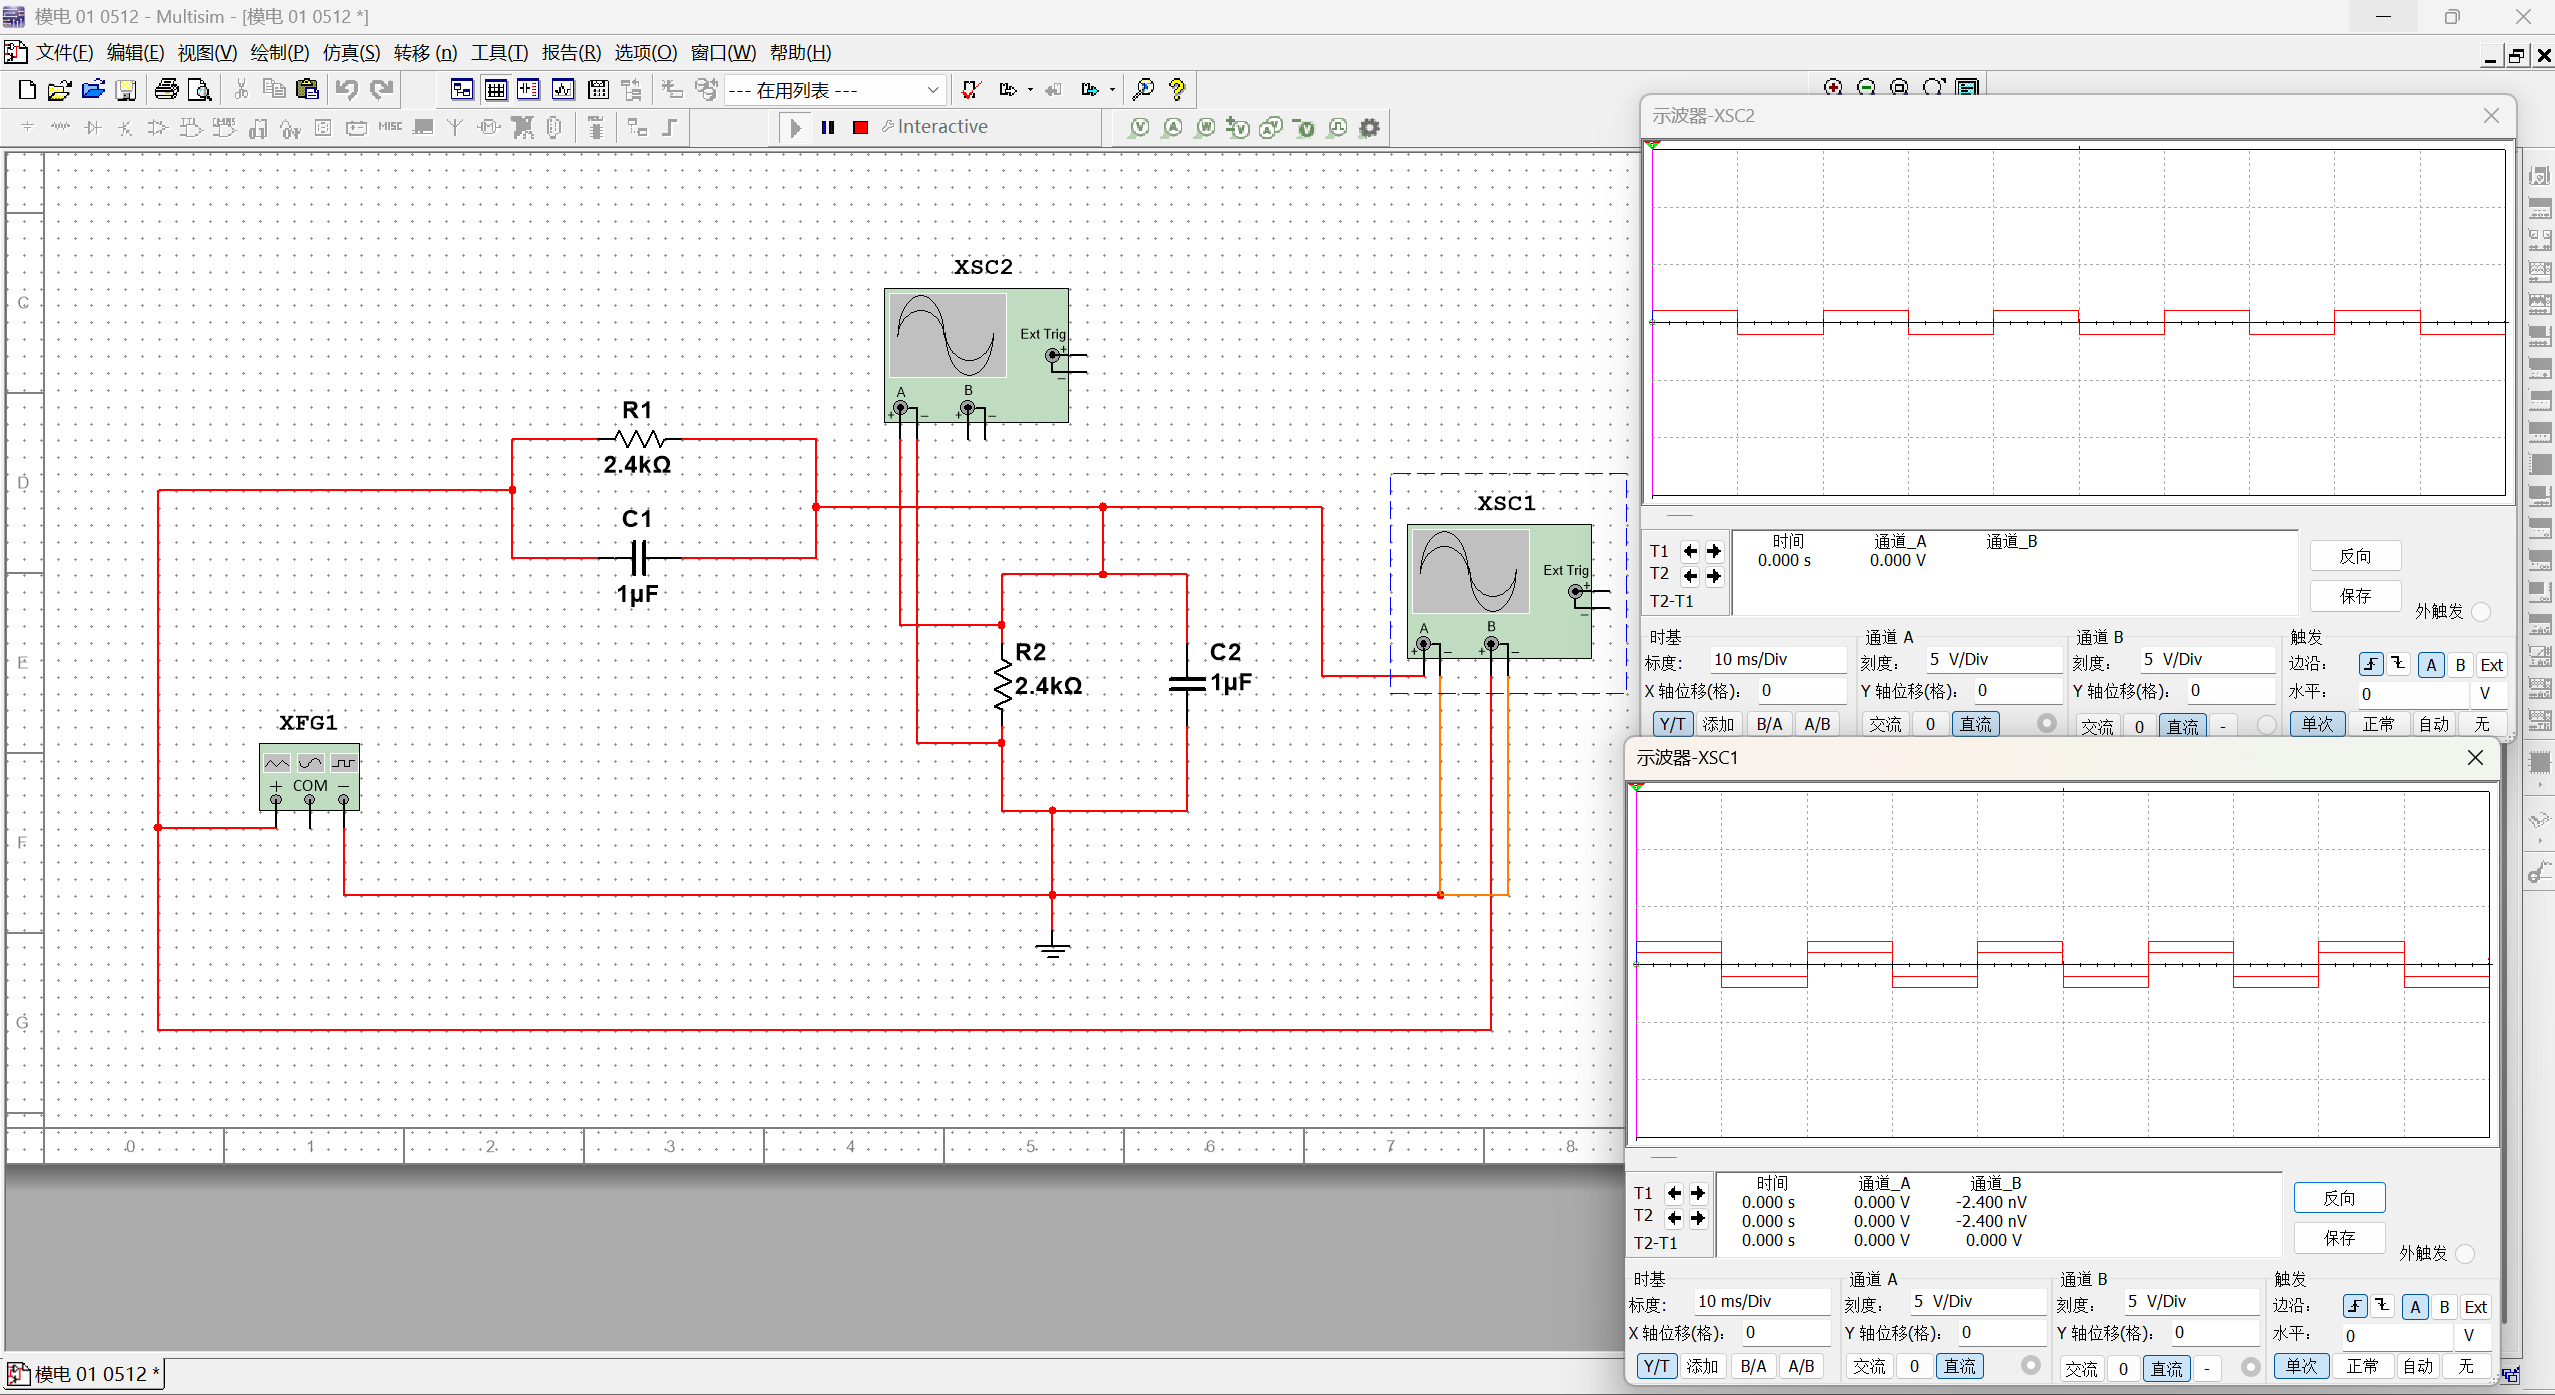
\includegraphics[width=1\textwidth]{fig_time_nodistort.png} 
    \caption{}
    \label{fig:time_nodistort}
\end{figure}


\begin{figure}[H]
    \centering
    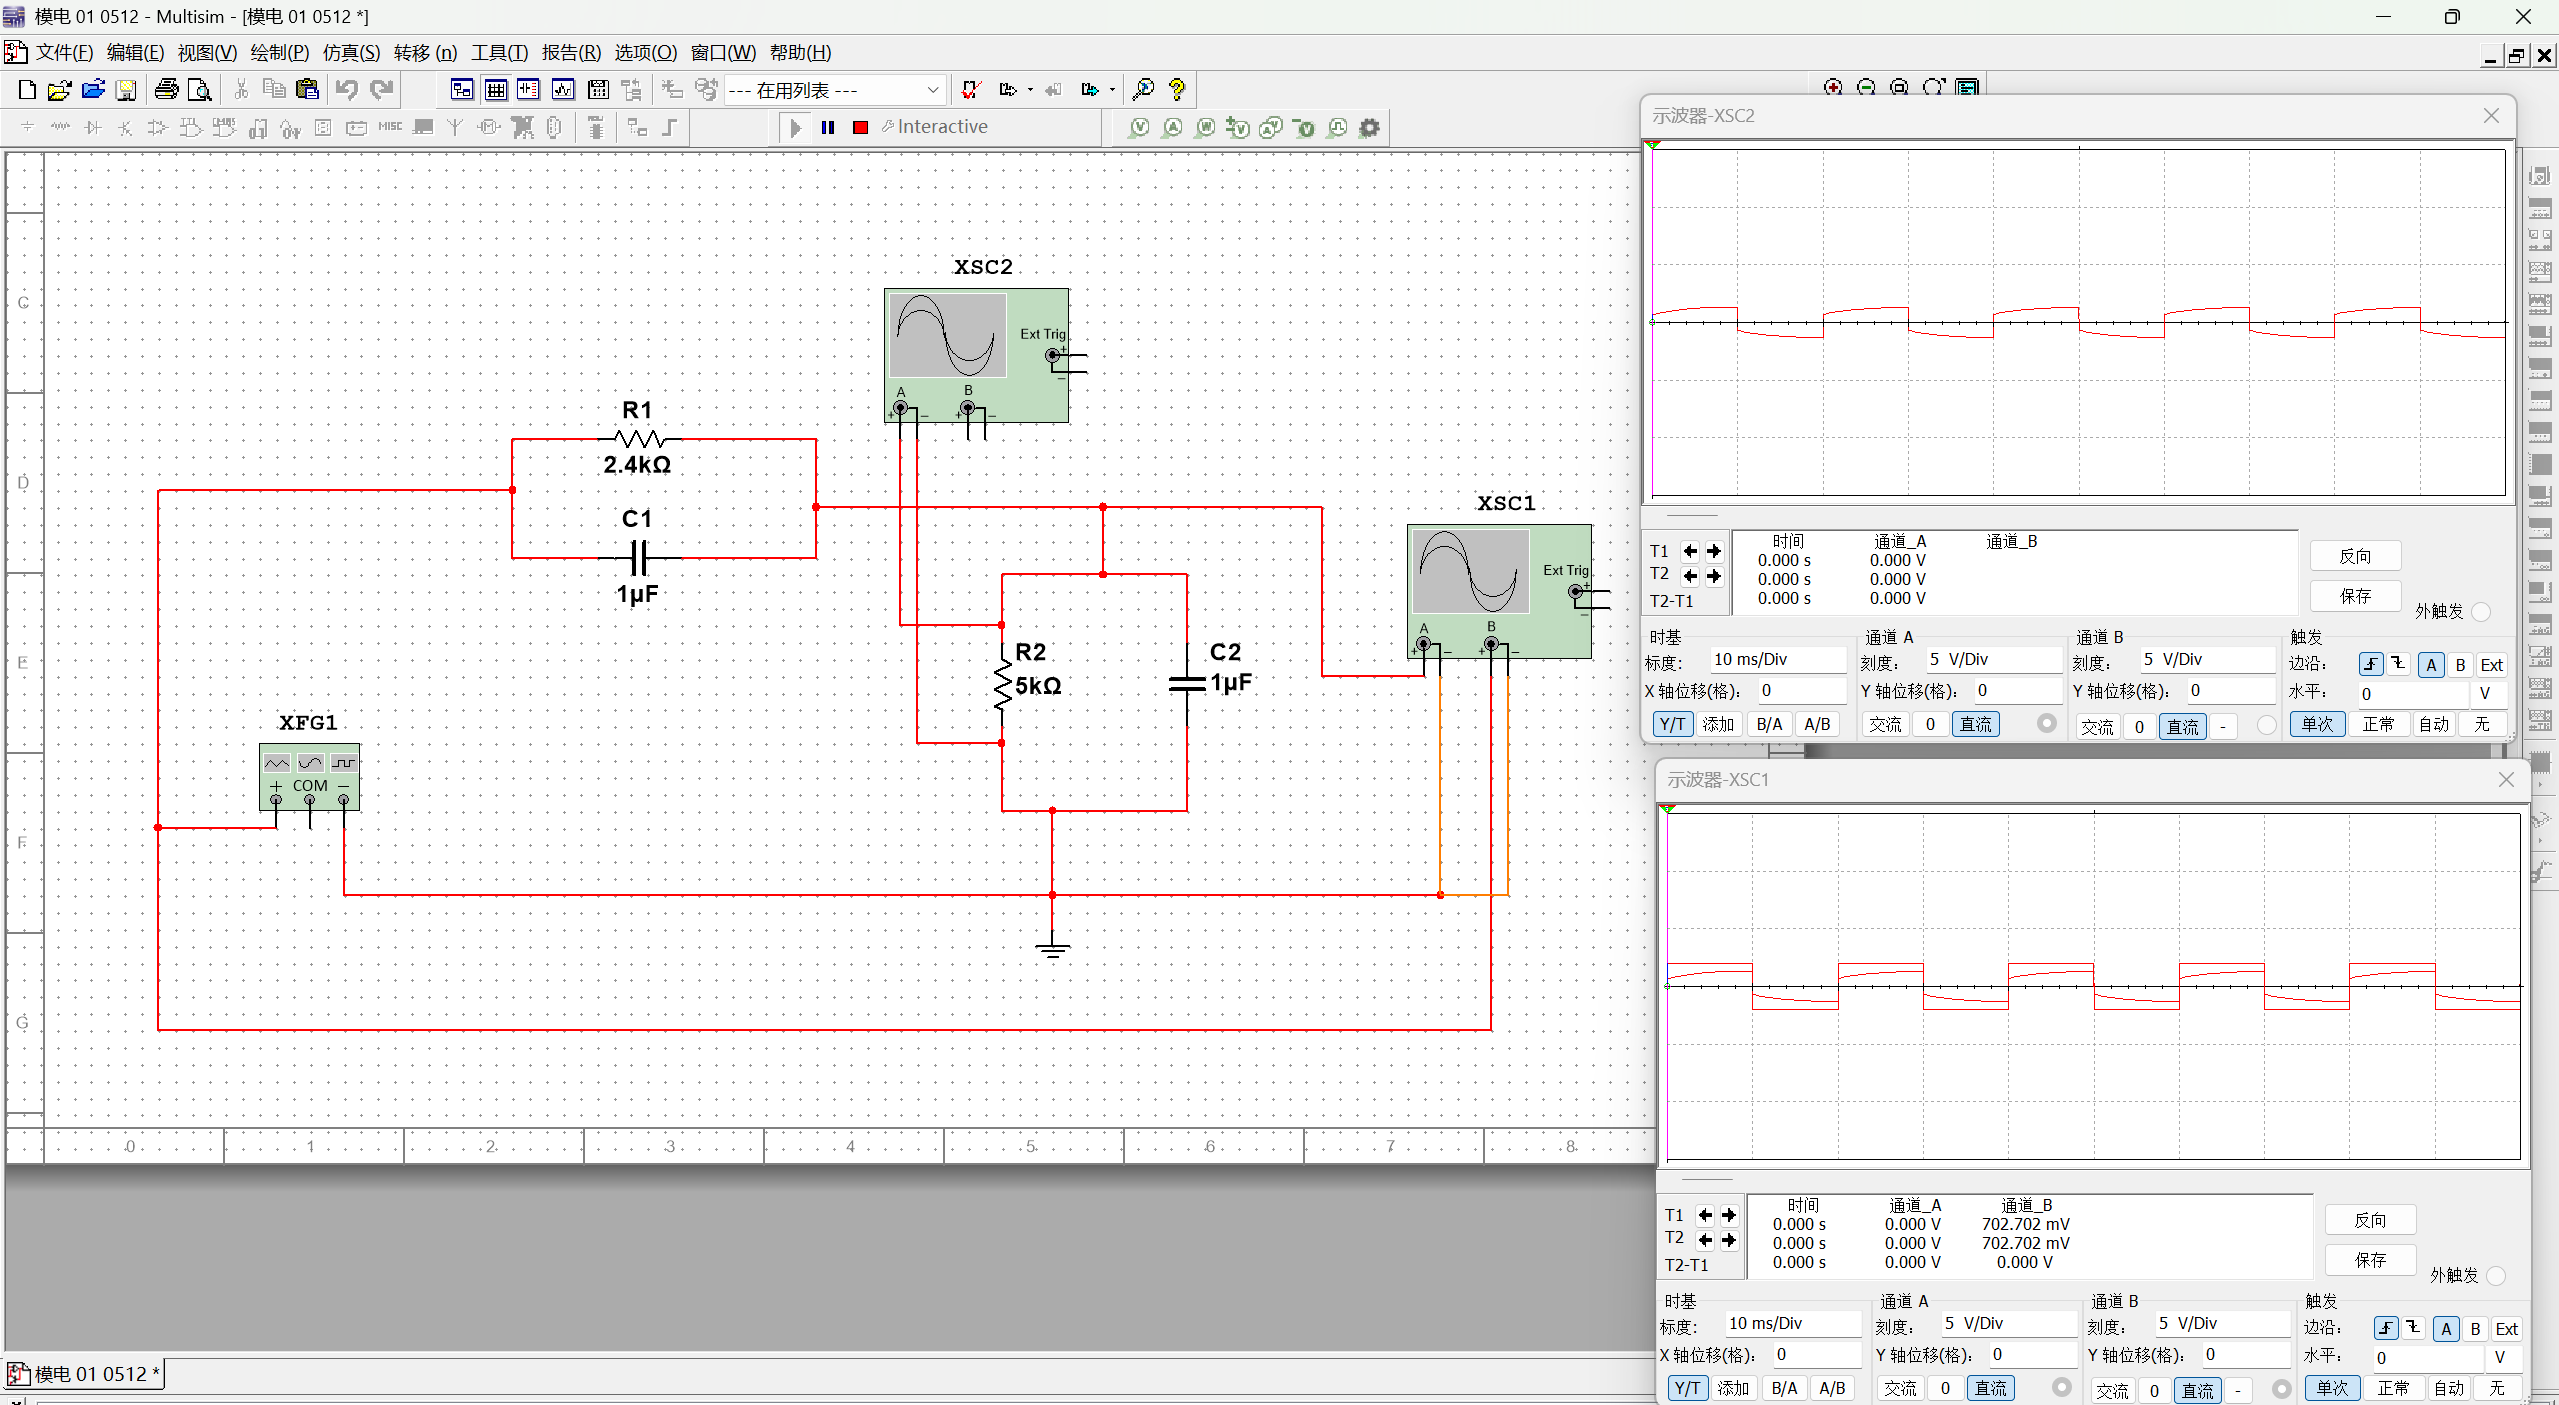
\includegraphics[width=1\textwidth]{fig_time_distort.png} 
    \caption{}
    \label{fig:time_distort}
\end{figure}

\subsection{第二题频响特性分析与关联}
通过交流分析（AC Sweep）获得的波特图如下
\begin{figure}[H]
    \centering
    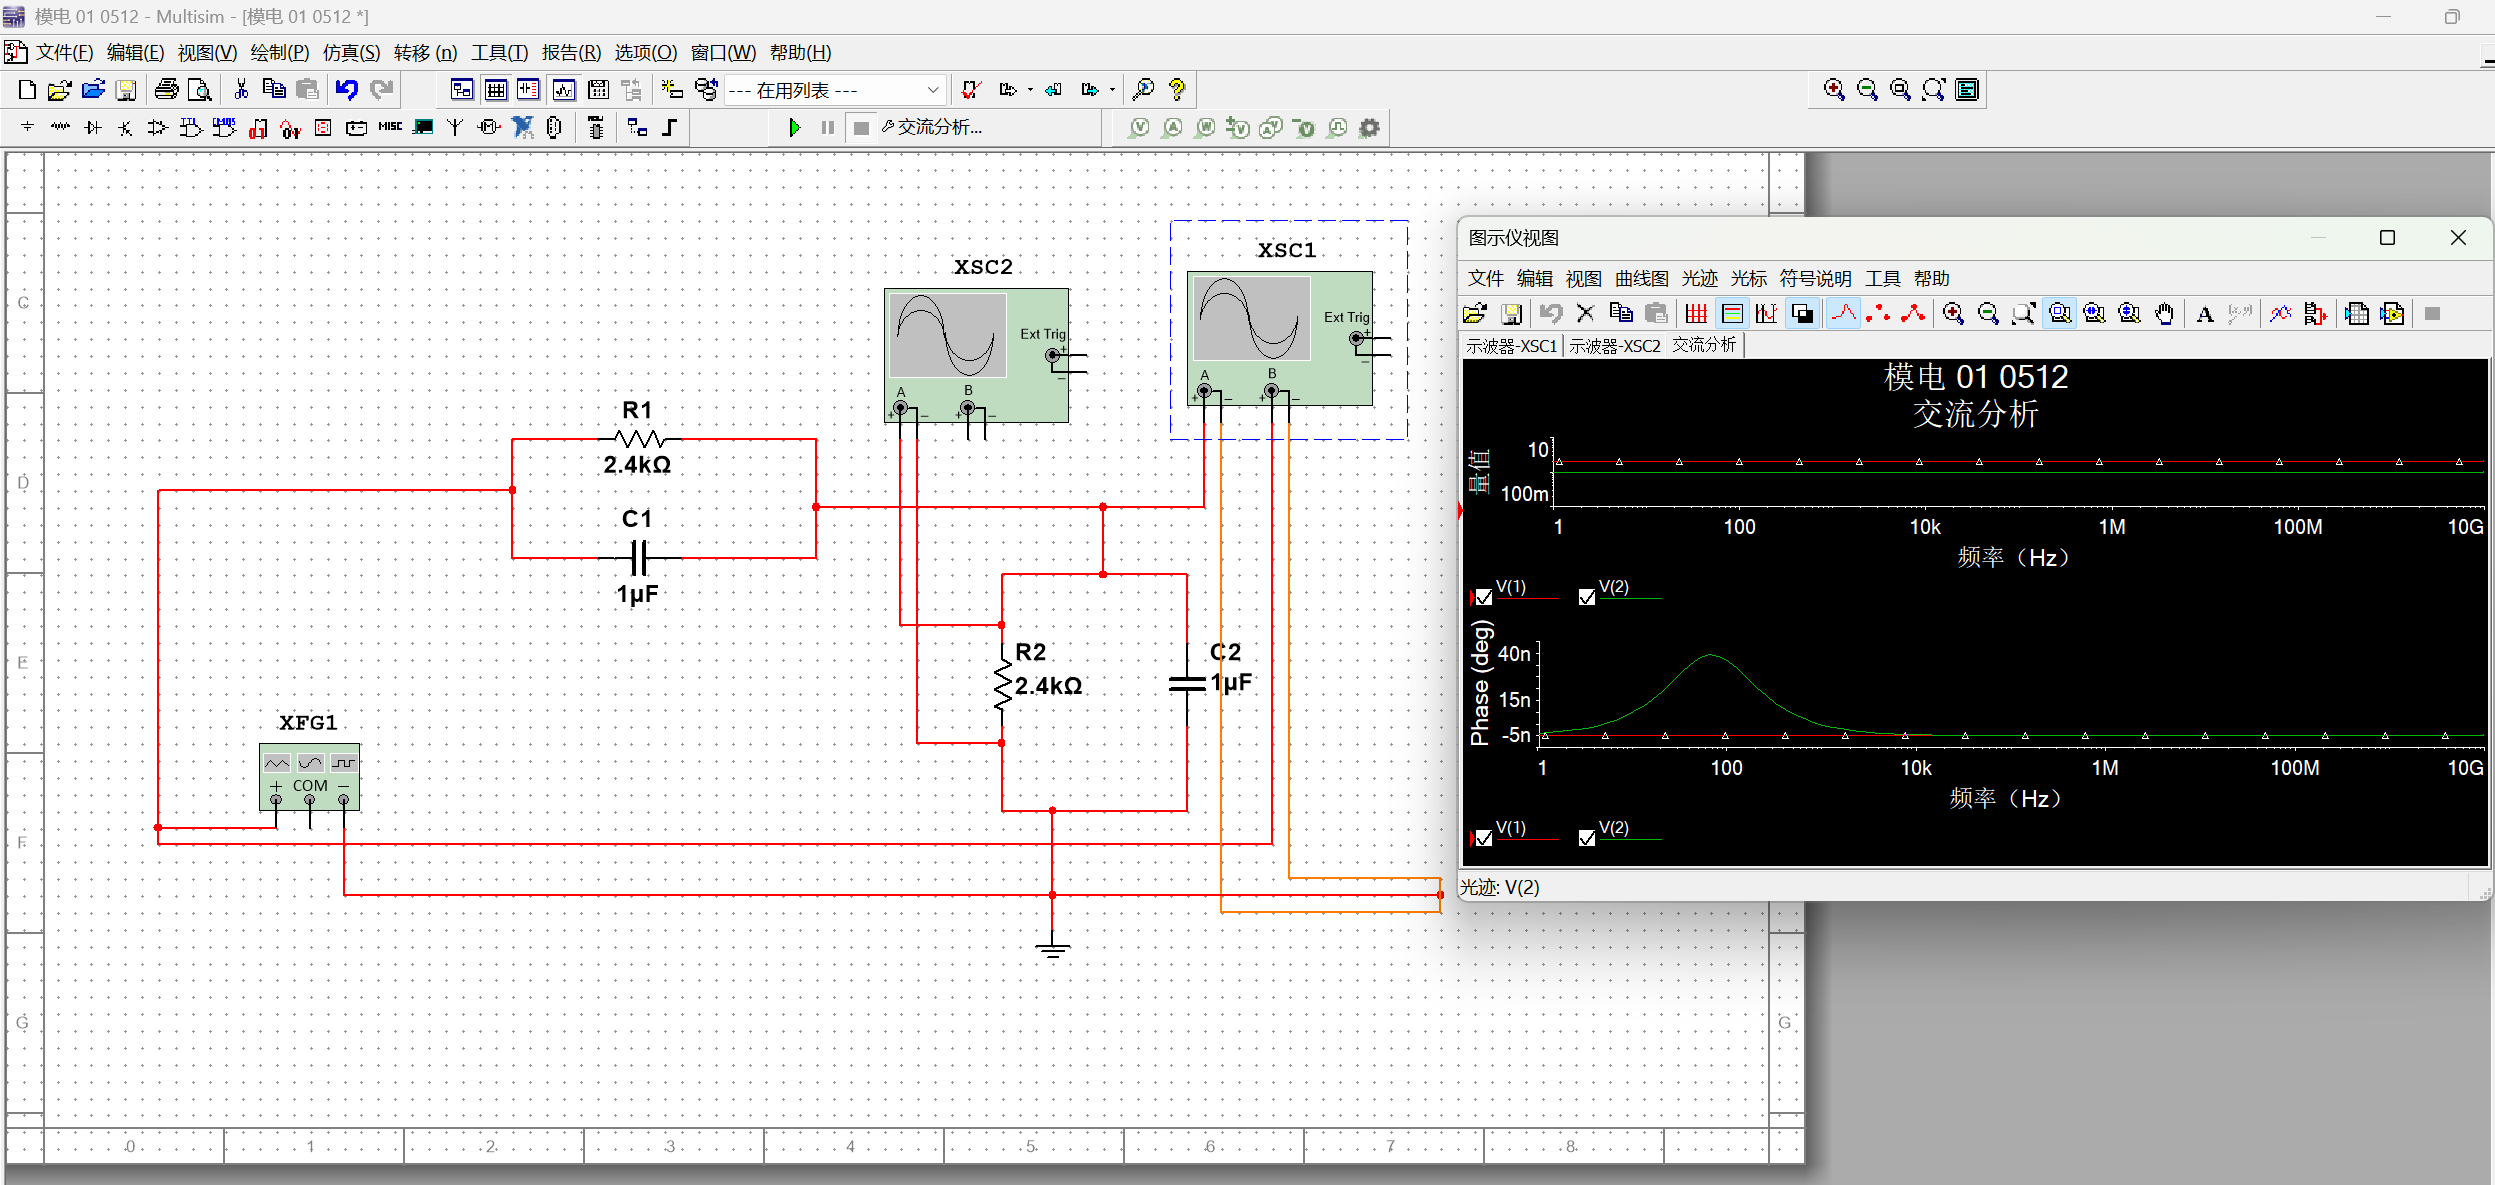
\includegraphics[width=1\textwidth]{fig_ac_sweep.png} 
    \caption{系统的幅频与相频特性曲线}
    \label{fig:ac_sweep}
\end{figure}
\textbf{波形失真原因} \\
频响特性曲线极大地帮助了我们理解时域中的方波失真。方波之所以失真，是因为它包含了丰富的宽频带谐波成分。从波特图可以看出，在失真条件下，系统对 $50\text{Hz}$ 以上的频率呈现出明显的低通滤波特性（高频衰减严重，且相位非线性）。方波的陡峭边缘依赖于高频谐波来维持，当这些高频成分被系统“滤除”或“延迟不一”时，时域上自然表现为边沿变缓、平顶倾斜，即发生了严重的线性失真。

\subsection{附加题全局参数扫描分析（$R_2$ 参数变化）}
为了分析电阻 $R_2$ 变化对系统的影响，我们在仿真中设置 \texttt{.param R2\_val}，并使用 Value List 方式选取了三个测试值（$1.2\text{k}\Omega, 2.4\text{k}\Omega, 4.8\text{k}\Omega$）。
\begin{figure}[H]
    \centering

    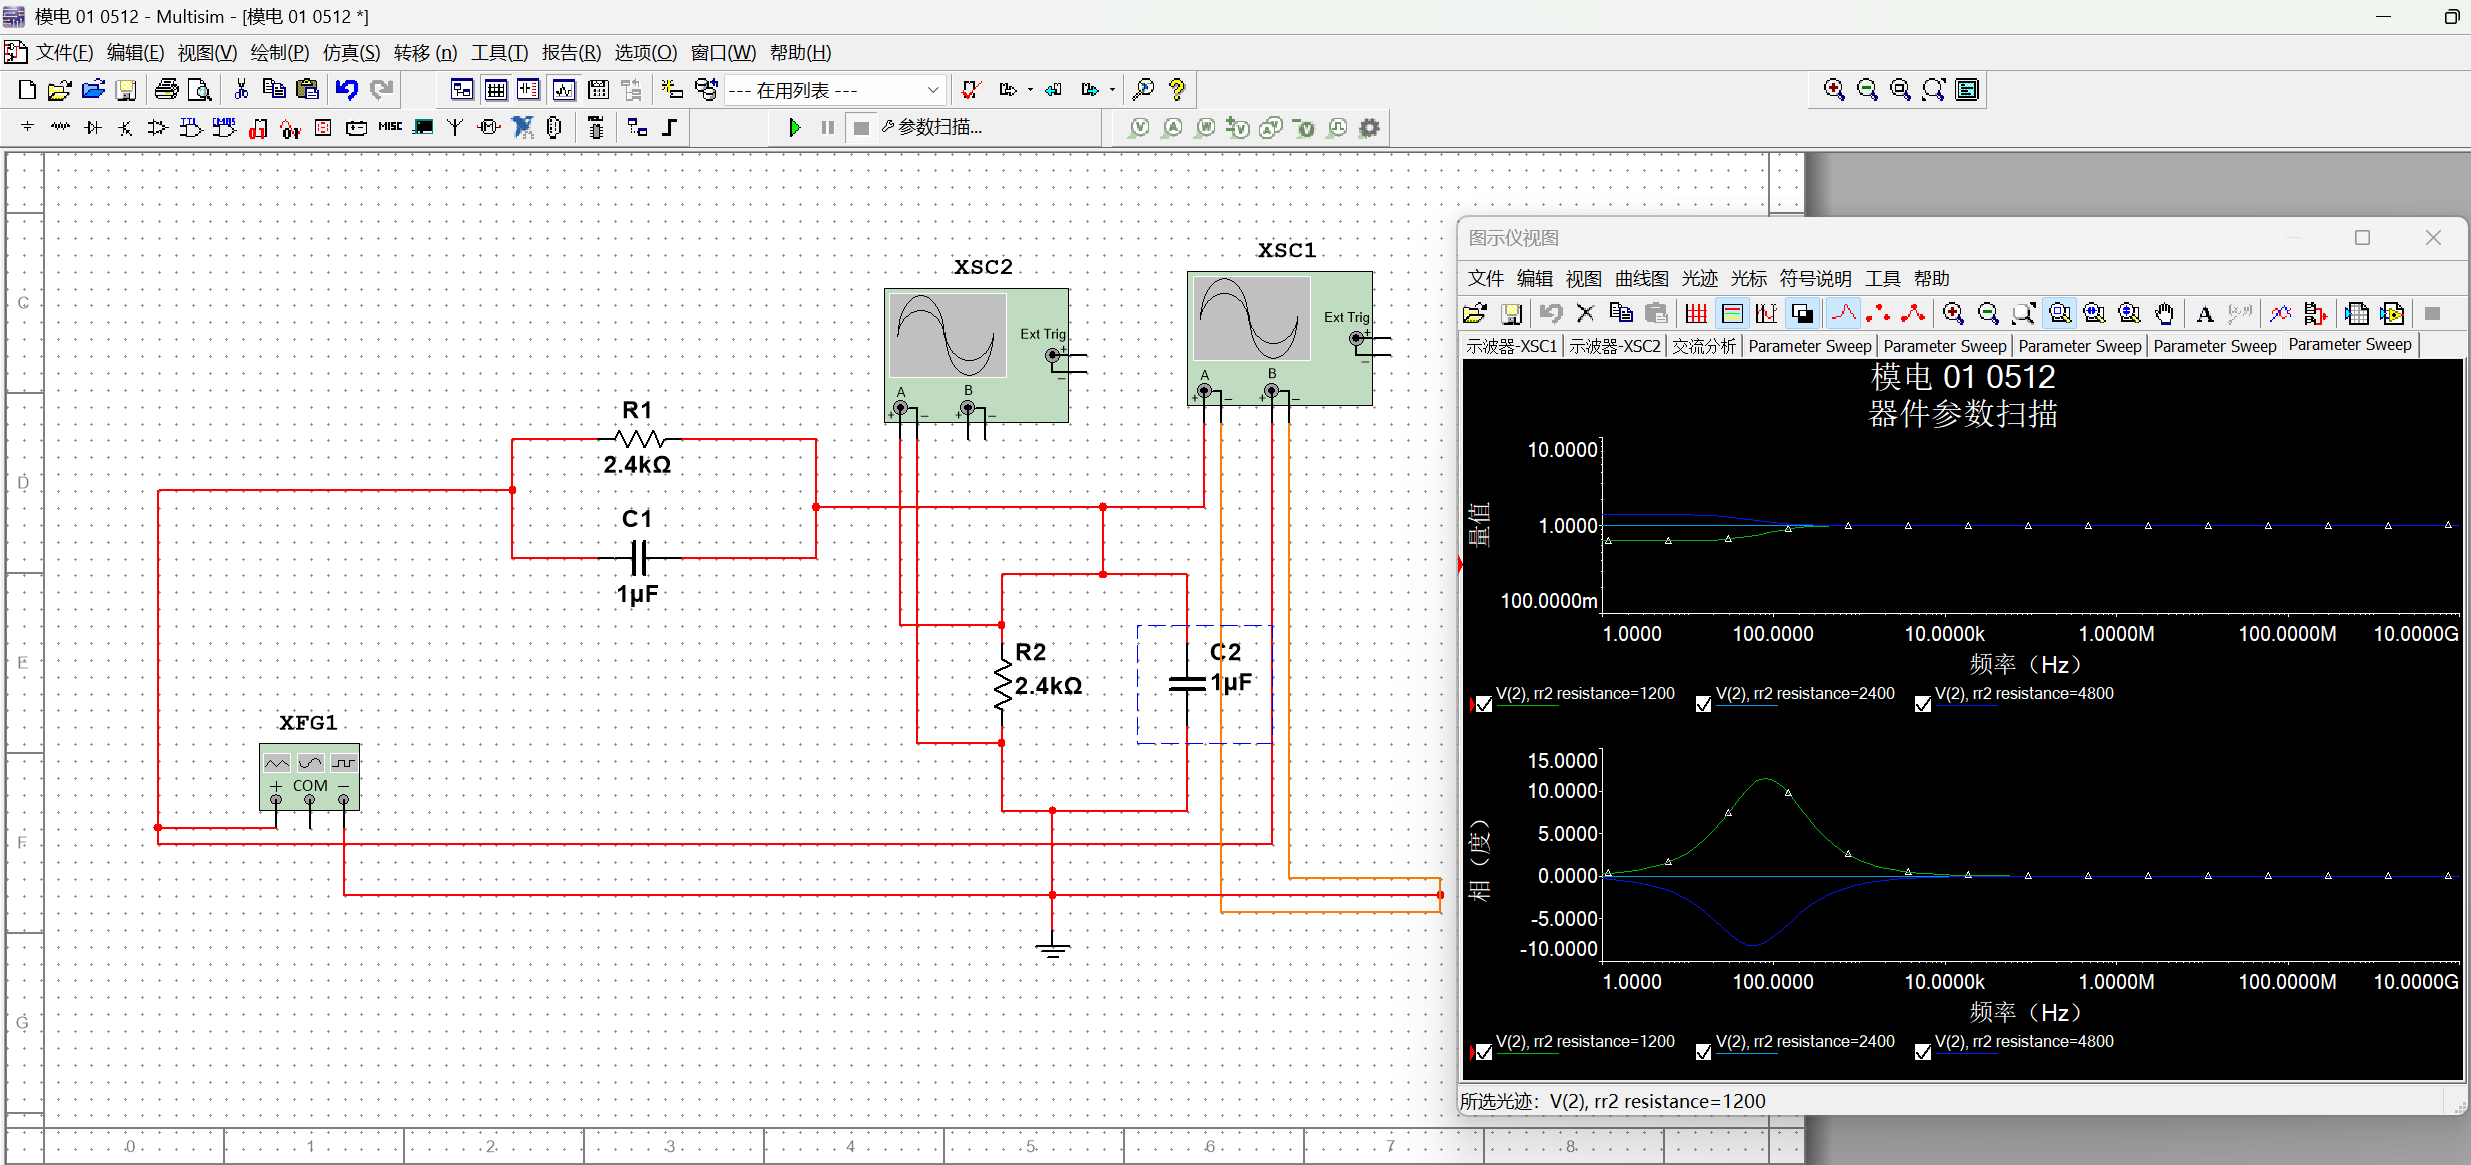
\includegraphics[width=1\textwidth]{fig_param_sweep.png} 

    \caption{$R_2$ 变化时的频响特性参数扫描曲线}
    \label{fig:param_sweep}
\end{figure}

\textbf{分析结论} $R_2$ 值的变化直接改变了系统的 RC 时间常数（基准在 $2.4\text{k}\Omega \times 1\mu\text{F} \approx 2.4\text{ms}$）。随着 $R_2$ 的增大，截止频率向低频方向移动，系统的高频抑制能力增强。在时域上表现为方波输出的上升沿更加平缓，充放电时间延长，失真程度加剧。

% ==========================================
% 第二部分：数字电路
% ==========================================
\newpage
\section{第二部分数字电路基于 74LS00 的三人表决器设计}

\subsection{实验目的}
\begin{enumerate}
    \item 掌握组合逻辑电路的设计流程：从需求分析、列真值表到化简逻辑表达式。
    \item 熟练运用 74LS00芯片实现特定的逻辑功能。
    \item 掌握在 Multisim 环境下的数字电路搭建、逻辑转换器使用及仿真验证方法。
\end{enumerate}

\subsection{实验原理与逻辑推导}
三人表决器规则为：少数服从多数，即 3 人中有 $\geq 2$ 人同意（输入为 1）时，表决通过（输出为 1），否则不通过。

\textbf{1. 真值表} 设输入为 $A, B, C$，输出为 $F$。
\begin{table}[H]
    \centering
    \caption{三人表决器真值表}
    \begin{tabular}{ccc|c}
        \toprule
        $A$ & $B$ & $C$ & $F$ \\
        \midrule
        0 & 0 & 0 & 0 \\
        0 & 0 & 1 & 0 \\
        0 & 1 & 0 & 0 \\
        0 & 1 & 1 & 1 \\
        1 & 0 & 0 & 0 \\
        1 & 0 & 1 & 1 \\
        1 & 1 & 0 & 1 \\
        1 & 1 & 1 & 1 \\
        \bottomrule
    \end{tabular}
\end{table}

\textbf{2. 逻辑表达式推导}
由真值表写出最小项表达式并化简得到“与或”式
$$F = AB + BC + AC$$
由于实验限制使用 74LS00根据摩根定律进行“与非-与非”转
$$F = \overline{\overline{AB + BC + AC}} = \overline{\overline{AB} \cdot \overline{BC} \cdot \overline{AC}}$$
由于 74LS00 只有 2 输入，实现三变量与非需级联：$F = \overline{ \overline{\overline{AB}\cdot\overline{BC}} \cdot \overline{AC} }$，共需使用两片 74LS00（6个与非门单元）。

\subsection{Multisim 仿真步骤}
\begin{enumerate}
    \item 调用两片 74LS00N 芯片、3 个交互式数字常量开关（作为输入 $A, B, C$）和 1 个 PROBE LED 指示灯（作为输出 $F$）。
    \item 按照转换后的与非逻辑表达式完成原理图接线。
    \item 接入 Multisim 逻辑转换器（Logic Converter），将其输入接 $A,B,C$，输出接 $F$。
    \item 运行仿真，手动拨动开关遍历 8 种组态，观察 LED 状态并记录。
\end{enumerate}

\subsection{仿真图与测试验证}
\textbf{ Multisim 电路原理图}
\begin{figure}[H]
    \centering
    % 请将准备好的电路原理图命名为 fig_logic_circuit.png 并替换下面的文件名
    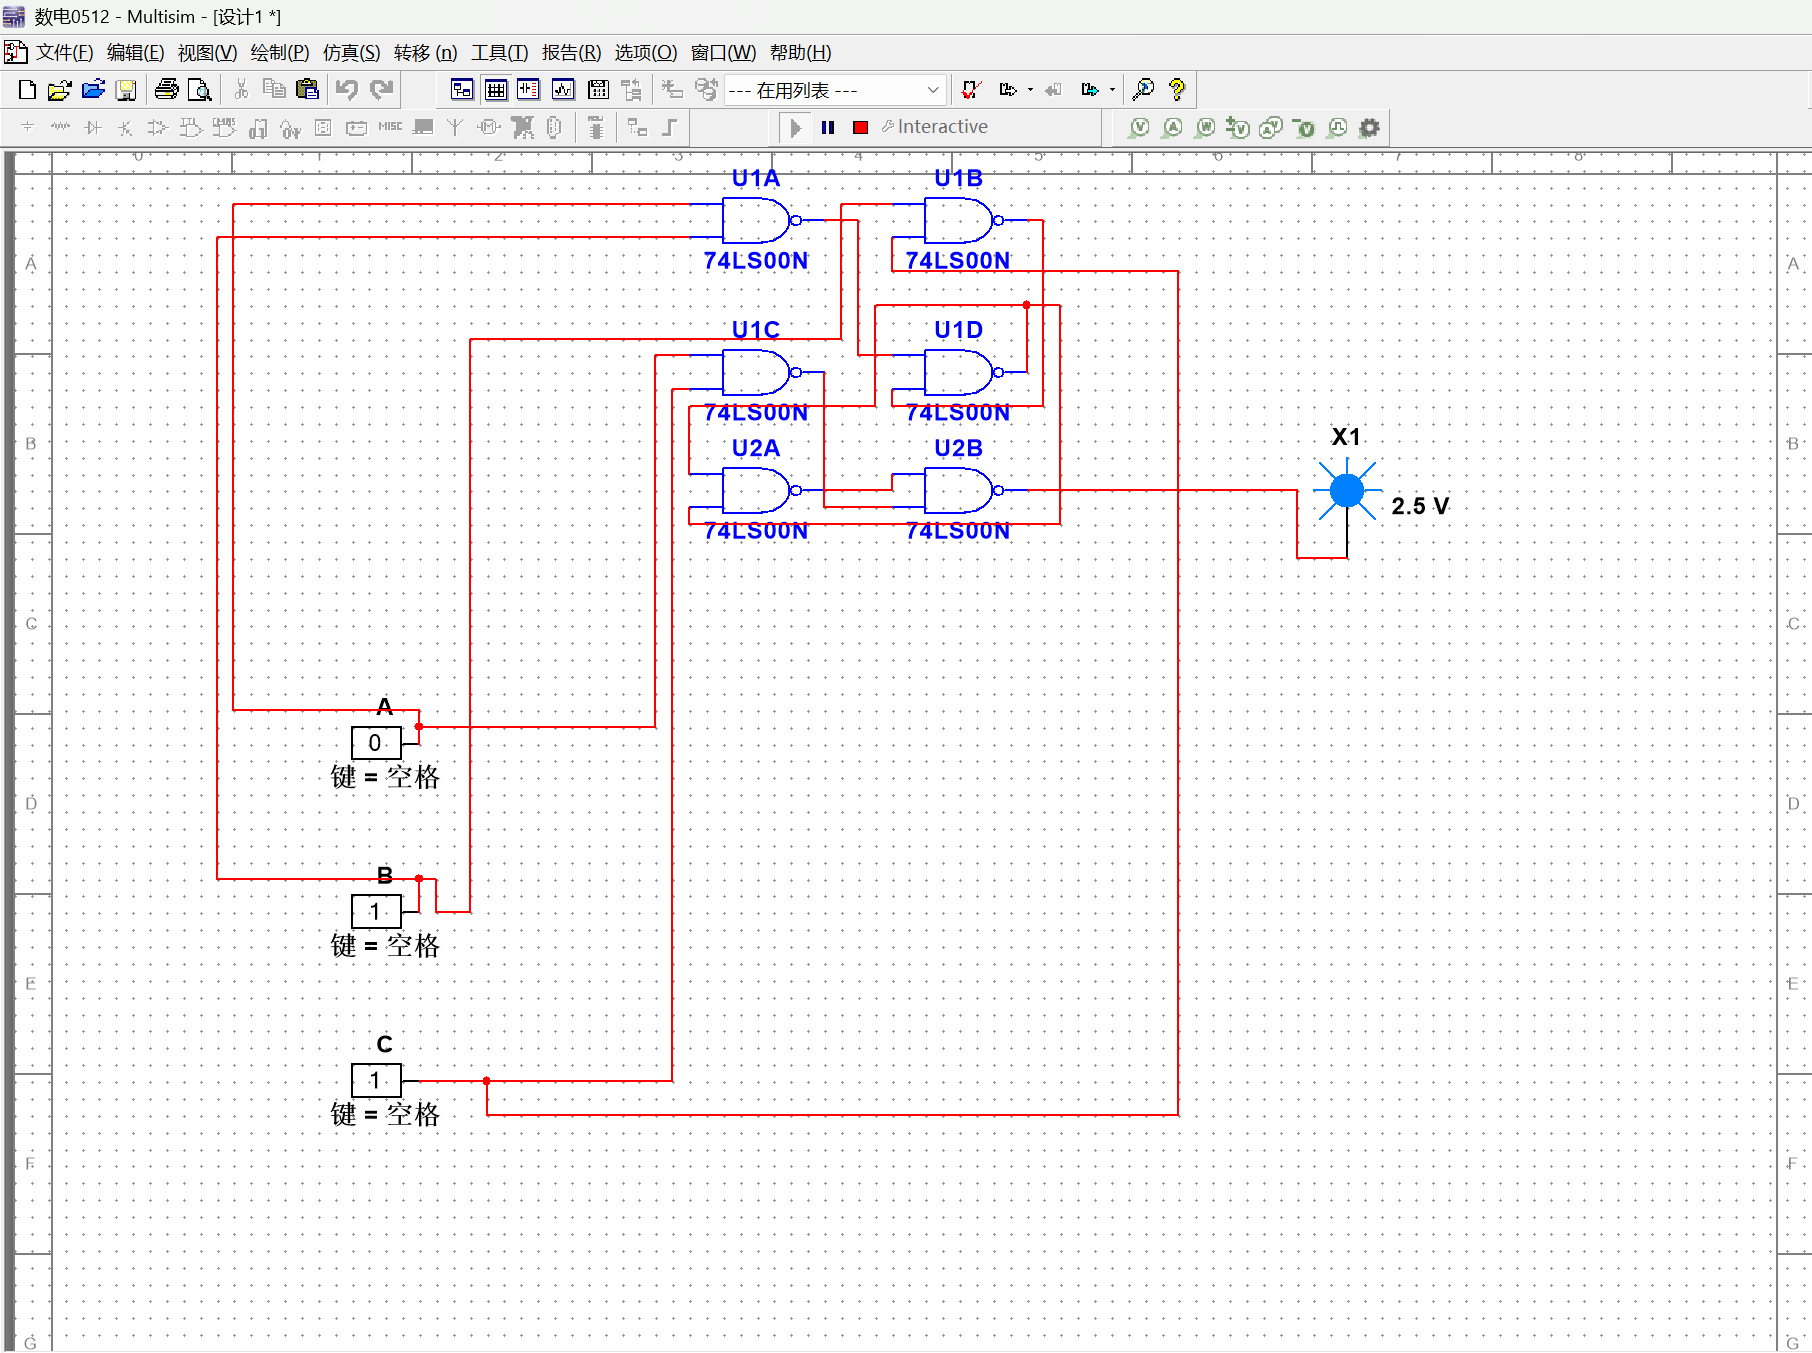
\includegraphics[width=1\textwidth]{fig_logic_circuit.png} 
    \caption{基于 74LS00 的三人表决器 Multisim 仿真图}
    \label{fig:logic_circuit}
\end{figure}

\textbf{真值表与逻辑验证结果}
经过逐一组态测试，LED 的亮灭情况与理论真值表完全吻合，逻辑功能正确。
\begin{figure}[H]
    \centering
    % 请将准备好的逻辑转换器/真值表截图命名为 fig_logic_truth.png 并替换下面的文件名
    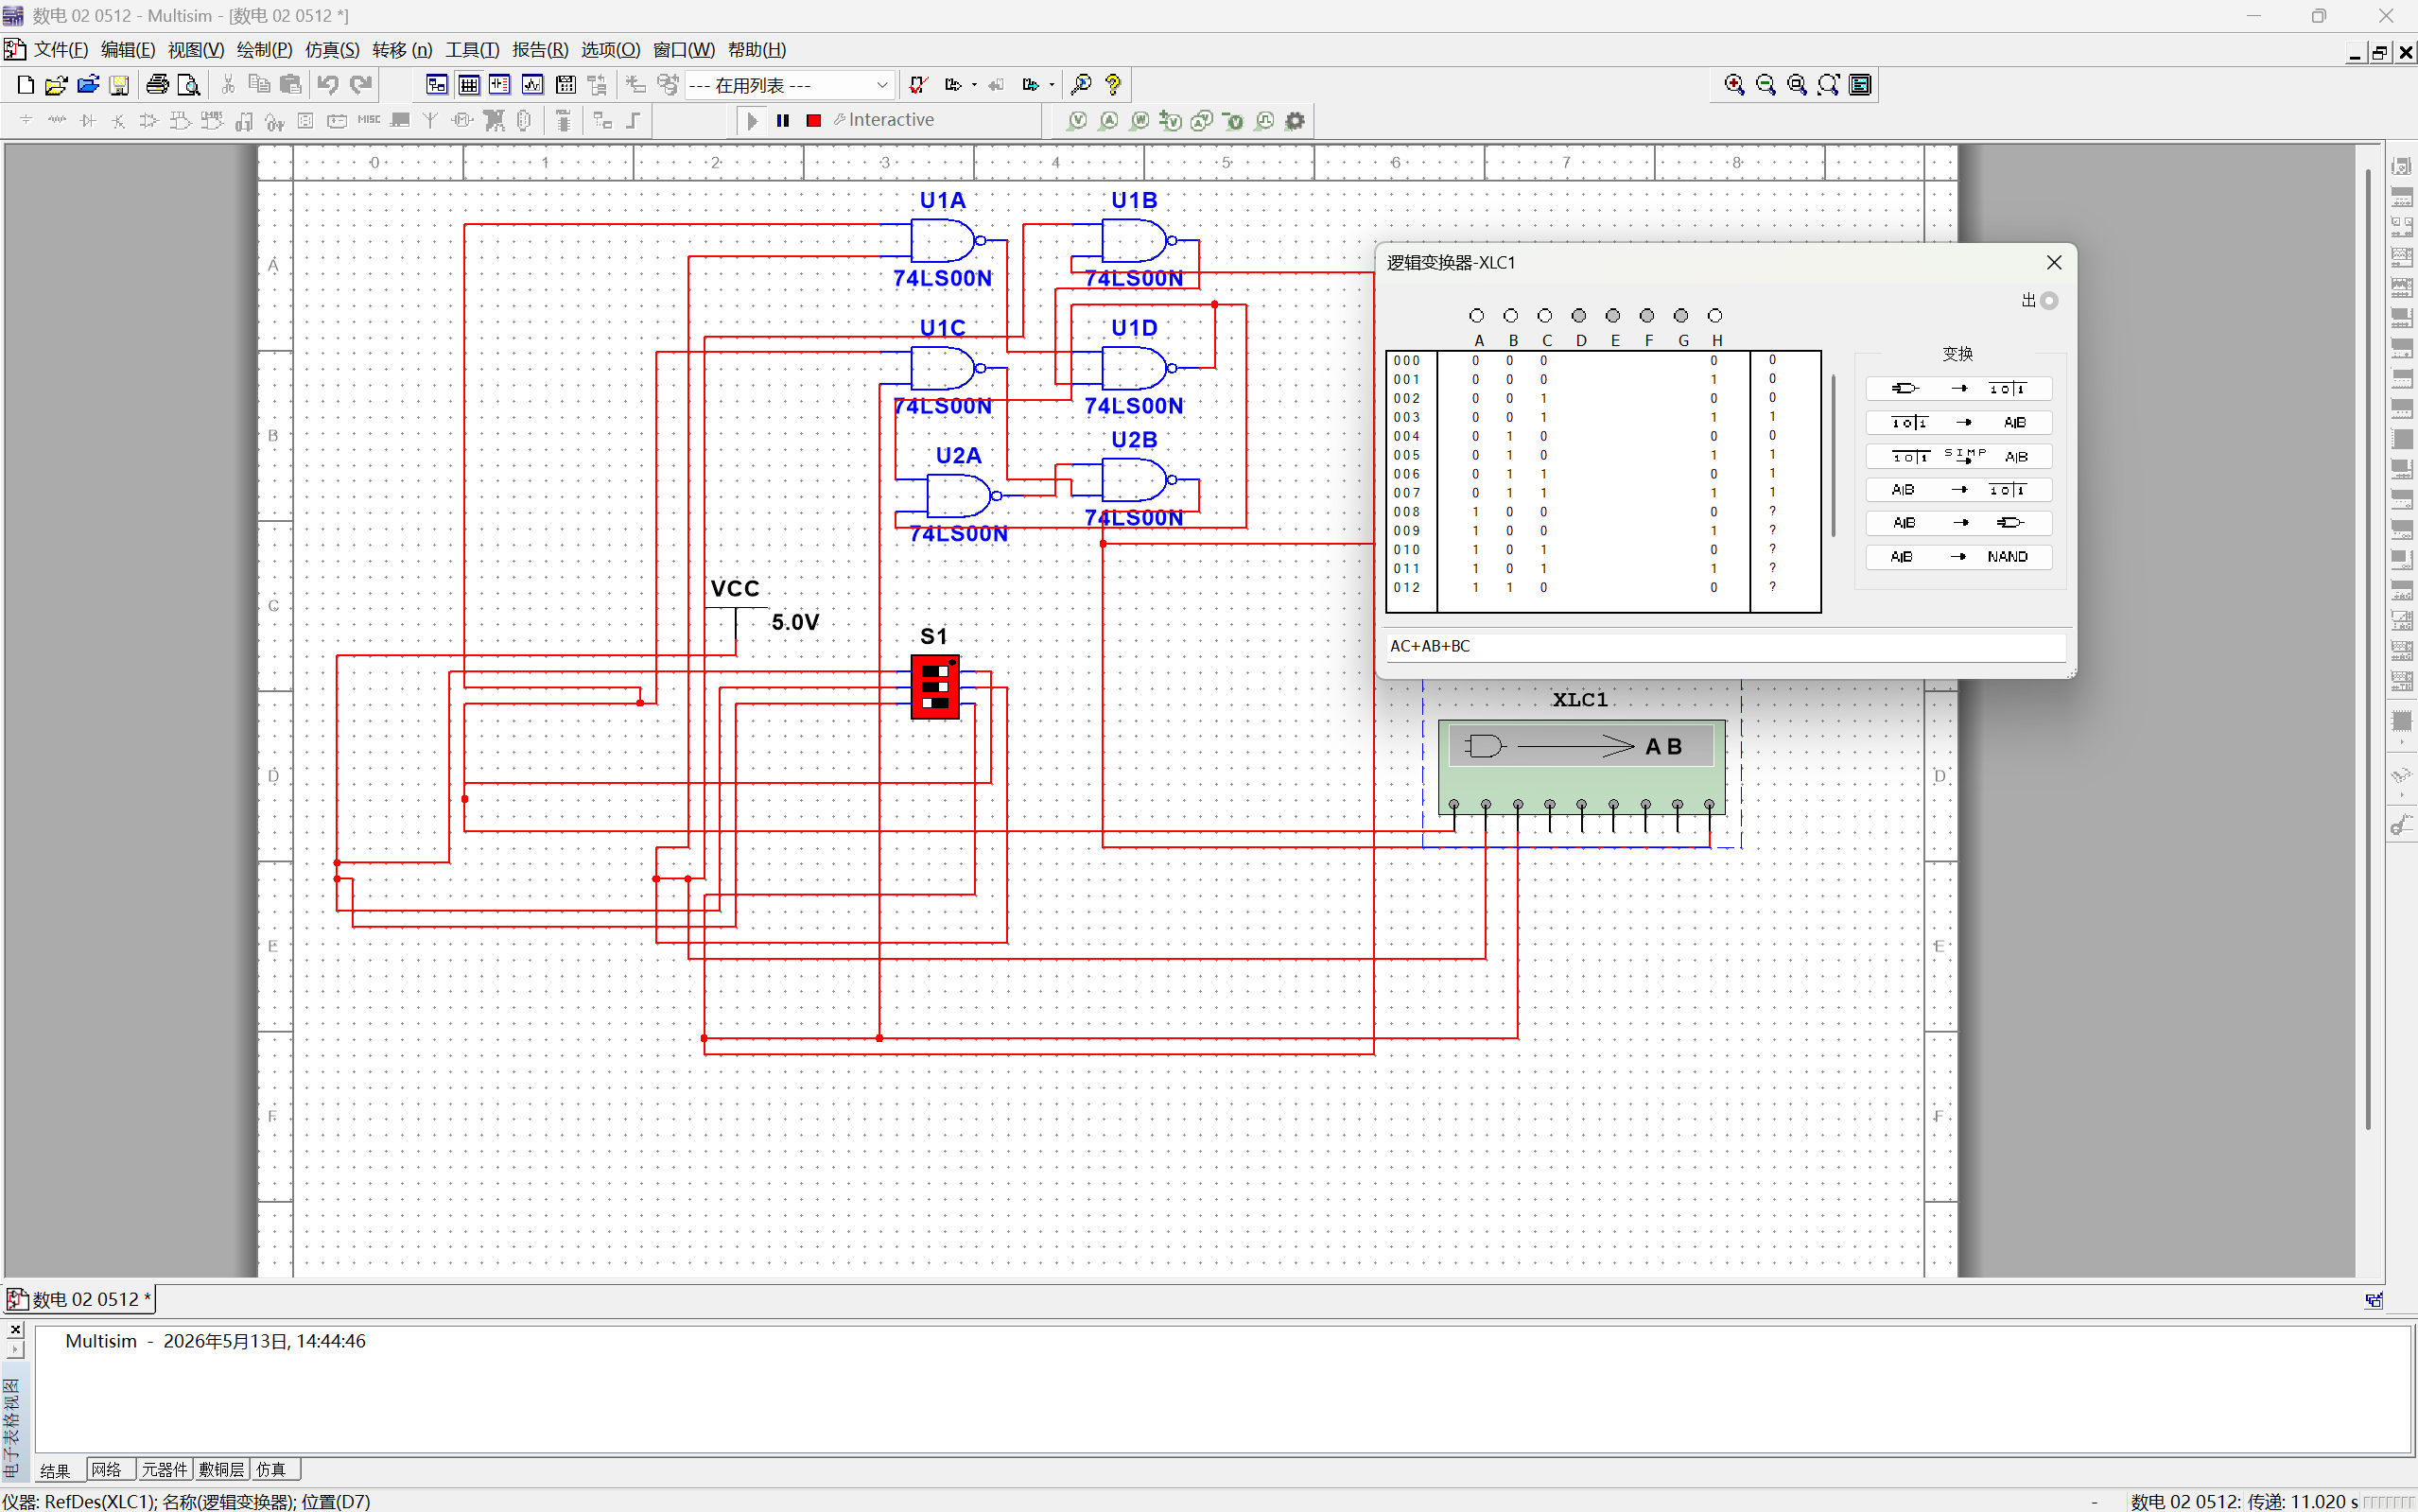
\includegraphics[width=1\textwidth]{fig_logic_truth.png} 
    \caption{逻辑转换器自动生成的真值表验证结果}
    \label{fig:logic_truth}
\end{figure}

\subsection{异常记录原因及解决方案}
\begin{table}[H]
    \centering
    \caption{仿真异常与排故记录表}
    \begin{tabular}{p{3.5cm}p{5cm}p{6cm}}
        \toprule
        \textbf{异常现象} & \textbf{原因分析} & \textbf{解决方案} \\
        \midrule
        接线完毕后，LED 无论输入何种状态均常亮或微闪。 
        & 74LS00 为 TTL 电路，仿真中部分闲置输入引脚悬空，TTL 悬空相当于输入高电平，导致内部逻辑状态不确定或紊乱。 
        & 检查原理图，将所有用作“非门”的与非门（如 U2A），其两个输入端必须短接在一起再接入前级输出，不可悬空一个引脚。 \\
        \midrule
        高速瞬态分析时，输出端出现极窄的毛刺（竞争冒险）。 
        & 信号通过不同路径到达最后一级与非门的延迟时间不一致（门电路传输延迟差）。 
        & 若在实际电路中，可在输出端并联微小电容（如 $100\text{pF}$）进行滤波；仿真中可在波形上标注不影响稳态逻辑。 \\
        \bottomrule
    \end{tabular}
\end{table}

\section{综合总结}
本次实验涵盖了从模拟系统的频域特性到数字逻辑设计的全流程分析。在模拟部分，通过时域和频域的结合，直观地揭示了信号频谱畸变导致时域失真的微观机制，并通过参数扫描功能验证了系统带宽与波形保真度之间的矛盾关系。在数字部分，成功将抽象的布尔代数逻辑转化为底层的与非门硬件实现，不仅验证了摩根定律的有效性，也通过 Multisim 平台的交互式仿真暴露并解决了 TTL 引脚悬空的细节问题，深化了对理论结合实践的理解。

\end{document}